% ---------------------------------------------------------------------
\section{$A$, $B$, $C$ and what they mean (new figures)}

\Q What does each invariant mean, and why is the capacity the one that disappears?

\D Both figures come from \texttt{fig\_abc.py} and the repository's model code at the
Table~\rn{new.tab.params} constants $\theta=\rn{calc.theta}$, $K_m=\rn{calc.Km}$,
$k_e=\rn{calc.ke}$, $\bar m=\rn{calc.mbar}$, $D=\rn{calc.D}$, $T=\rn{calc.T}$~d,
$t_{1/2}=\rn{calc.thalf}$~d, $L=\theta g(\bar m)+k_e\bar m=\rn{calc.L}$. The balance
$L+b=(\theta+\Delta)m/(K_m+m)+k_e m$ gives $\Delta(m)=A/m+B+Cm$, $A=K_m(L+b)$,
$B=L+b-\theta-k_eK_m$, $C=-k_e$.

\F Every check value reproduces: $A=\rn{calc.A}$, $B=\rn{calc.B}$, $C=\rn{calc.C}$, untreated
$m=\rn{calc.m_untreated}$, $\Delta(\rn{calc.mwf})=\rn{calc.delta6}$.\footnote{The check value
supplied for $\Delta(\rn{calc.mwf})$ disagrees with the repository; the repository's value is
printed, and the closing list records it.} At $\theta=\rn{calc.theta_dis}$:
$B=\rn{calc.B_dis}$, untreated $m=\rn{calc.m_untreated_dis}$, a ratio of
$\rn{calc.m_ratio_dis}$, matching the $\rn{lnew.scope_5pct_ratio}\times$ of
Table~\rn{new.tab.scope}. The twin at $b=\rn{calc.twin_b_last}$: $\theta=\rn{calc.twin400_theta}$,
$K_m=\rn{calc.twin400_km}$, relaxation $\rn{calc.relax_b400}$ against
$\rn{calc.relax_b0}$~d$^{-1}$, the paper's own two values in \S\rn{new.sec.collapse}
($\rn{lnew.relax_b400}$, $\rn{lnew.relax_b0}$).

\begingroup\footnotesize\centering
\begin{minipage}[t]{0.38\textwidth}\vspace{0pt}
\centering
\begin{tabular}{@{}lcccl@{}}
\toprule
parameter & $A$ & $B$ & $C$ & reading \\
\midrule
$\theta$ & & $\bullet$ & & own enzyme \\
$K_m$ & $\bullet$ & $\bullet$ & & half-saturation \\
$k_e$ & & $\bullet$ & $\bullet$ & backup route \\
$b$ & $\bullet$ & $\bullet$ & & diary error \\
\bottomrule
\end{tabular}
\end{minipage}\hfill
\begin{minipage}[t]{0.59\textwidth}\vspace{0pt}
\begin{tabularx}{\textwidth}{@{}lL@{}}
\toprule
invariant & what it is, and its size \\
\midrule
$A=K_m(L+b)$ & load $\times$ half-saturation: $+\rn{calc.A_over_6}$ at
$m=\rn{calc.mwf}$, the largest term \\
$B=L+b-\theta-k_eK_m$ & the only place $\theta$ appears: at $\theta=\rn{calc.theta_dis}$ the
smallest of $+\rn{calc.Bp_load}$, $-\rn{calc.theta_dis}$, $-\rn{calc.keKm}$, the scope limit of
\S\rn{new.sec.scopeprec} \\
$C=-k_e$ & the backup route: bend $\rn{calc.bend}$ over $m=\rn{calc.m_lo}$ to
$\rn{calc.m_hi}$ against $\rn{calc.diary_move}$ per $\rn{calc.unit_b}\,\mu$M/d of diary error,
so $k_e$ comes from a prior \\
\bottomrule
\end{tabularx}
\end{minipage}\par\endgroup

\begin{figure}[htbp]
\centering
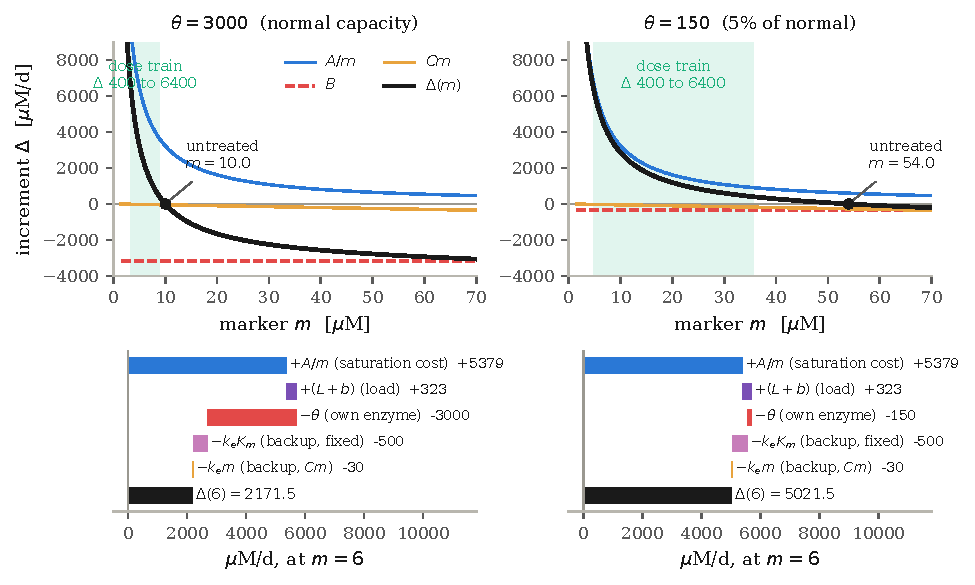
\includegraphics[width=0.80\textwidth]{fig5a_abc}
\caption{$\Delta(m)$ decomposed at $\theta=\rn{calc.theta}$ (left) and $\rn{calc.theta_dis}$
(right). Green: the dose train's range, $\Delta$ from $\rn{calc.trough}$ to $\rn{calc.peak}$.
Below, a waterfall at $m=\rn{calc.mwf}$: $A$ blue, $B$'s pieces purple, red, pink, $C$ amber.
$-\theta$ is $B$'s largest piece at normal capacity, its smallest at $\rn{calc.dis_pct}\%$.}
\label{fig:abc}
\end{figure}

\begin{figure}[htbp]
\centering
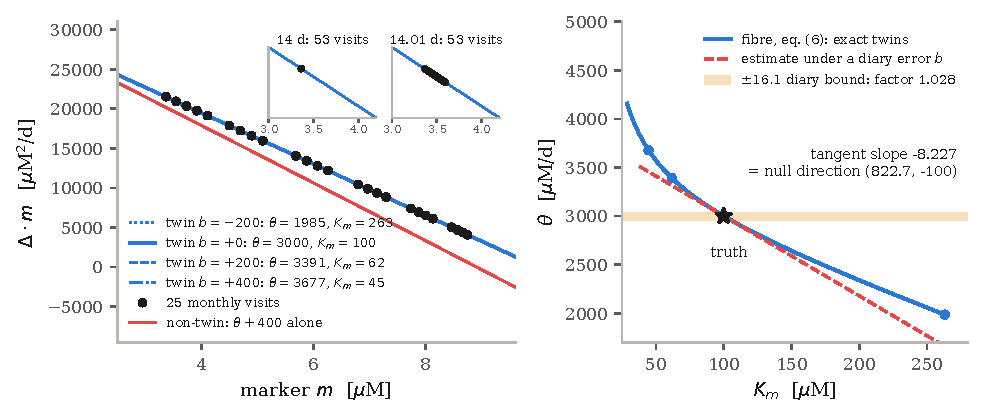
\includegraphics[width=0.80\textwidth]{fig5b_fibre}
\caption{Left: the record as a parabola, $\Delta m = A+Bm+Cm^2$. The \rn{calc.n_monthly}
monthly visits and the twins at $b\in\{\rn{calc.twin_bs}\}$ draw one curve; moving $\theta$
alone by $\rn{calc.nontwin_dtheta}$ does not. Insets: the aliased designs, one point every
$\rn{calc.T}$~d, a cluster every $\rn{new.near_step}$~d. Right: the fibre is curved, but
estimates under a constant diary error, $\hat K_m=K_m(1+b/L)$,
$\hat\theta=\theta-b(1+K_mk_e/L)$, lie on a line of slope $\rn{calc.locus_slope}$, tangent at
the truth along the rank proposition's null vector
$(\rn{calc.null_theta},\rn{calc.null_km})$. Shaded: the $\pm\rn{calc.diary_b}$ bound from the
$\rn{calc.load_pct}\%$ diary record, a factor of $\rn{calc.diary_factor}$ on $\theta$.}
\label{fig:fibre}
\end{figure}

\W Nothing: the increment law, the fibre and the invariants read the same in both drafts. The
27 Sept \S\rn{new.sec.destroys} adds the affine map $\hat\theta=\theta-\rn{new.bias_slope}\,b$
and the Vandermonde reading of the invariants. \textbf{The tangent reading is in neither
draft:} Figure~\ref{fig:fibre} puts estimates under a constant diary error on the fibre's
tangent at the truth, the rank proposition's null direction. One sentence for
\S\rn{new.sec.destroys}:
\begin{quote}\small
``The fibre is curved in $(K_m,\theta)$, but a constant load bias moves the estimate along its
tangent at the truth, Proposition~\textbackslash ref\{prop:rank\}'s null direction, so a bound
on $b$ leaves a segment of that tangent and the factor on $\theta$ is exact, not linearised.''
\end{quote}

\Out{$\theta$ lives in one invariant, beside two larger terms in the disease range: the scope
limit in a line of algebra.}
